\section{Introduction}
\label{sec:introduction}
In computational science, one wishes to resolve the physics around complex geometries (see e.g. \figref{fig:introAirfoil}).
To do so, one must divide the computational space into computational cells.
In the case of complex geometries, people frequently use an unstructured grid, consisting of triangles.
In order not to introduce too large of a numerical error as a consequence of the used grid, these triangles
must satisfy certain conditions.
I.e., the triangles should not have too large of a surface area,
since in that case we cannot fully resolve all relevant scales.
Also, the triangles should be as close to an equilateral triangle as possible, such that we can
properly approximate the gradients of quantities on boundaries of adjacent cells without resorting to expensive algorithms.
The latter condition is frequently translated to the requirement that the minimum angle
within any triangle should be above a certain criterion.


\begin{figure}
    \centering
    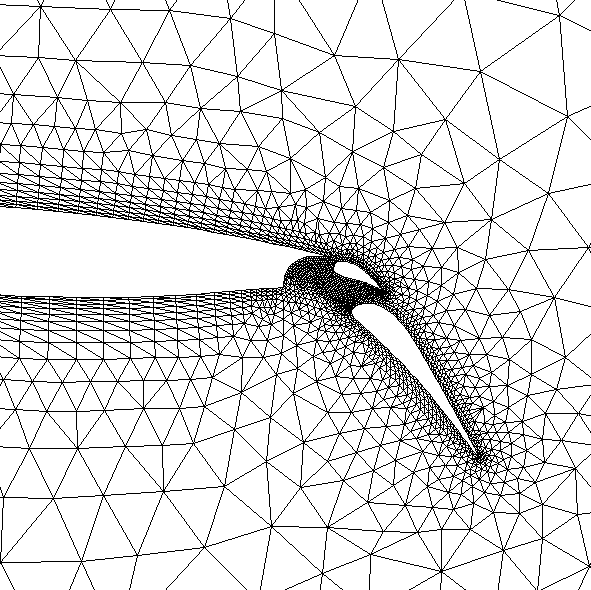
\includegraphics[width=\columnwidth]{../images/airfoil.png}
    \caption{Example of an unstructured grid around some airfoils consisting of solely triangles \cite{img:airfoilImage}.}
    \label{fig:introAirfoil}
\end{figure}

In this report, we will analyse several Delaunay triangulation and refinement algorithms
in terms of their complexity and runtime.
In the case of the triangulation algorithms, the problem is given by a set of points and the goal is to find the Delaunay triangulation belonging to that set of points.
%In the case of the triangulation algorithms, the problem is given by ``given a set of points,
%find the Delaunay triangulation belonging to that set of points''.
Furthermore, the solution can be constrained by a set PSLG (plane straight line graph) of
boundary vertices, which may not be crossed and whose edges must occur in the solution.

For the refinement algorithms the input is specified as a set of PSLG boundary vertices and
the goal is to triangulate the area with triangles with a certain minimum quality while respecting the boundary.
%For the refinement algorithms the problem is given by ``given a set of PSLG (plane straight line graph)
%boundary vertices, triangulate the area with triangles with a certain minimum quality while respecting the boundary''.
The Delaunay refinement algorithms that we will discuss are build on top of a Delaunay triangulation algorithm.

A Delaunay triangulation (as introduced by Delaunay in 1934 \cite{art:Delaunay1934}) is defined as follows:

% FIXME T = D!!
``Given a set of vertices $P = \{p_1 \ldots p_n\}$, a Delaunay triangulation, $D$, is a triangulation, $T$, of $P$
iff for each triangle $t \in T$ the circumcircle contains no vertex $p \in P$ in its interior.''
In our definition, it is allowed for other vertices to lie on the circumcircle, which imposes an ambiguity on $D$
when more than three points like on the same circle. In this case, any permutation of $D$ will do.

Another way to define the Delaunay triangulation is as the dual graph of the Voronoi diagram.
If we let $cell(p_i)$ be the points in $P$ that are closer to $p_i$ than to any other point of $P$,
those cells together form the Voronoi diagram of $P$.

Firstly, we will look at the Delaunay triangulation algorithms.
Afterwards, we will look at refinement algorithms.
%TODO: Mention names of algorithms in order.


